\documentclass[ignorenonframetext]{beamer}
\usepackage[orientation=portrait,size=a0,scale=1.5]{beamerposter}
\usepackage{textpos}

\usetheme{Berlin}
\setbeamercovered{transparent}
\setbeamertemplate{bibliography item}[text]

\beamertemplatenavigationsymbolsempty

\addtobeamertemplate{block end}{}{\vspace*{2ex}} % White space under blocks
\addtobeamertemplate{block alerted end}{}{\vspace*{2ex}} % White space under highlighted (alert) blocks
\setlength{\belowcaptionskip}{2ex} % White space under figures
\setlength\belowdisplayshortskip{2ex} % White space under equations

\usepackage{newclude}
%\usepackage[british]{babel}
\usepackage{hyperref}
\usepackage{xparse}
\usepackage{booktabs}

\usepackage{interval}

\usepackage{csquotes}
%\usepackage[natbib,style=numeric-comp,maxbibnames=99]{biblatex}
\addbibresource{crypto.bib}
\addbibresource{location.bib}
\addbibresource{reputation.bib}
\addbibresource{auth.bib}
\addbibresource{voting.bib}
\addbibresource{protests.bib}
\addbibresource{blockchain.bib}
\addbibresource{anon.bib}
\addbibresource{ecurrency.bib}

\usepackage[capitalize]{cleveref}
\crefname{properties@i}{property}{properties}
\Crefname{properties@i}{Property}{Properties}
\crefname{requirements@i}{requirement}{requirements}
\Crefname{requirements@i}{Requirement}{Requirements}

\usepackage{tikz}
\usepackage{tikzscale}
\usetikzlibrary{arrows.meta}
\usepackage{tikz-qtree}

%\DeclareDocumentCommand{\keywords}{m}{%
%  \par
%  \textbf{Keywords:} #1
%}
\usepackage[operators,sets]{cryptocode}

\usepackage{bibsp}


\DeclareDocumentEnvironment{properties}{o}{%
  \begin{block}{Properties}
    \IfValueTF{#1}{\begin{enumerate}[{#1}1]}{\begin{enumerate}}
}{%
    \end{enumerate}
  \end{block}
}
\DeclareDocumentEnvironment{requirements}{o}{%
  \begin{block}{Requirements}
    \IfValueTF{#1}{\begin{enumerate}[{#1}1]}{\begin{enumerate}}
}{%
    \end{enumerate}
  \end{block}
}
\DeclareDocumentEnvironment{adversaries}{o}{%
  \begin{block}{Adversaries}
    \IfValueTF{#1}{\begin{enumerate}[{#1}1]}{\begin{enumerate}}
}{%
    \end{enumerate}
  \end{block}
}


\ProvideDocumentEnvironment{lightblock}{mm}{%
  \setbeamercolor{block body}{bg=#1!10,fg=black}
  \setbeamercolor{block title}{bg=#1,fg=black}
  \setbeamercolor{local structure}{fg=#1}
  \begin{block}{#2}
}{%
  \end{block}
}
\ProvideDocumentEnvironment{darkblock}{mm}{%
  \setbeamercolor{block body}{bg=#1!10,fg=black}
  \setbeamercolor{block title}{bg=#1,fg=white}
  \setbeamercolor{local structure}{fg=#1}
  \begin{block}{#2}
}{%
  \end{block}
}

\ProvideDocumentEnvironment{blackblock}{m}
{\begin{darkblock}{black}{#1}}
{\end{darkblock}}
\ProvideDocumentEnvironment{whiteblock}{m}{%
  \setbeamercolor{block body}{bg=white!10,fg=black}
  \setbeamercolor{block title}{bg=white,fg=black}
  \setbeamercolor{local structure}{fg=black}
  \begin{block}{#1}
}{%
  \end{block}
}
\ProvideDocumentEnvironment{bwblock}{m}{%
  \setbeamercolor{block body}{bg=white!10,fg=black}
  \setbeamercolor{block title}{bg=black,fg=white}
  \setbeamercolor{local structure}{fg=black}
  \begin{block}{#1}
}{%
  \end{block}
}

\ProvideDocumentEnvironment{redblock}{m}
{\begin{darkblock}{red}{#1}}
{\end{darkblock}}
\ProvideDocumentEnvironment{blueblock}{m}
{\begin{darkblock}{blue}{#1}}
{\end{darkblock}}
\ProvideDocumentEnvironment{purpleblock}{m}
{\begin{darkblock}{purple}{#1}}
{\end{darkblock}}

\ProvideDocumentEnvironment{greenblock}{m}
{\begin{lightblock}{green}{#1}}
{\end{lightblock}}
\ProvideDocumentEnvironment{yellowblock}{m}
{\begin{lightblock}{yellow}{#1}}
{\end{lightblock}}
\ProvideDocumentEnvironment{orangeblock}{m}
{\begin{lightblock}{orange}{#1}}
{\end{lightblock}}

\ProvideDocumentEnvironment{assumption}{o}{%
  \IfValueTF{#1}{%
    \begin{block}{Assumption: #1}
  }{%
    \begin{block}{Assumption}
  }
}{%
  \end{block}
}

\ProvideDocumentEnvironment{protocol}{o}{%
  \IfValueTF{#1}{%
    \begin{block}{Protocol: #1}
  }{%
    \begin{block}{Protocol}
  }
}{%
  \end{block}
}

\ProvideDocumentEnvironment{remark}{o}{%
  \IfValueTF{#1}{%
    \begin{alertblock}{Note: #1}
  }{%
    \begin{alertblock}{Note}
  }
}{%
  \end{alertblock}
}

\ProvideDocumentEnvironment{idea}{o}{%
  \IfValueTF{#1}{%
    \begin{block}{Idea: #1}
  }{%
    \begin{block}{Idea}
  }
}{%
  \end{block}
}

\ProvideDocumentEnvironment{question}{o}{%
  \setbeamercolor{block body}{bg=orange!15,fg=black}
  \setbeamercolor{block title}{bg=orange,fg=white}
  \setbeamercolor{local structure}{fg=orange}
  \IfValueTF{#1}{%
    \begin{block}{Question: #1}
  }{%
    \begin{block}{Question}
  }
}{%
  \end{block}
}

\ProvideDocumentEnvironment{exercise}{o}{%
  \setbeamercolor{block body}{bg=yellow!10,fg=black}
  \setbeamercolor{block title}{bg=yellow,fg=black}
  \setbeamercolor{local structure}{fg=yellow}
  \IfValueTF{#1}{%
    \begin{block}{Exercise: #1}
  }{%
    \begin{block}{Exercise}
  }
}{%
  \end{block}
}

\ProvideDocumentEnvironment{assumption}{o}{%
  \IfValueTF{#1}{%
    \begin{block}{Assumption: #1}
  }{%
    \begin{block}{Assumption}
  }
}{%
  \end{block}
}



\title{Securely and Privately Verifiable Protests}
\author{%
  Daniel Bosk <dbosk@kth.se>\inst{1}
  \and
  Sonja Buchegger\inst{1}
  \and
  Sébastien Gambs\inst{2}
}
\institute{%
  \inst{1}
  KTH Royal Institute of Technology, Stockholm,
  \and
  \inst{2}
  Université de Quebec à Montreal,
}

\begin{document}\begin{frame}[t]
  \begin{columns}
  \begin{column}{0.17\linewidth}
    
\includegraphics[width=0.5\linewidth]{fig/kth_cmyk.eps}
    \hfill
  \end{column}
  \hfill
  \begin{column}{0.64\linewidth}
    \begin{center}
      \Huge\bfseries
      Securely and Privately Verifiable Protests
    \end{center}
    \begin{center}
      \large
      Daniel Bosk <dbosk@kth.se>
      $\bullet$
      Sonja Buchegger
      $\bullet$
      Sébastien Gambs
    \end{center}
    \vspace{1.5em}
  \end{column}
  \hfill
  \begin{column}{0.17\linewidth}
    \hfill
    
\includegraphics[width=0.8\linewidth]{fig/uqam.pdf}
  \end{column}
\end{columns}

\begin{columns}[t]

  \begin{column}{0.32\linewidth}

    \begin{blueblock}{Scenario: The crowd-counting problem}
      \begin{itemize}
        \item Alice organizes a protest against Eve's regime.
        \item Bob, Carol and others show up.
        \item Must know how many showed up to support Alice's cause.
      \end{itemize}
    \end{blueblock}

    \begin{figure}
      \centering
      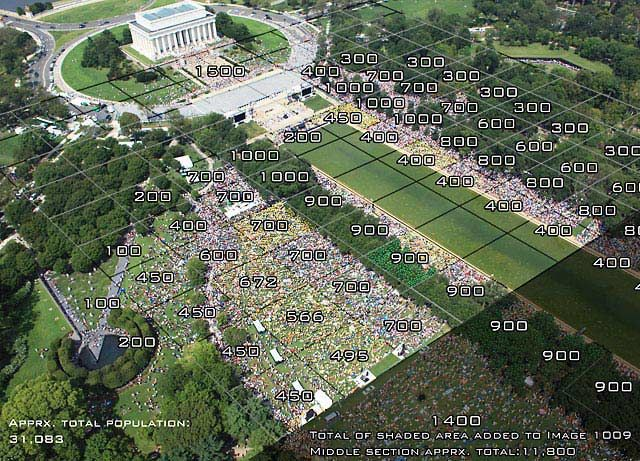
\includegraphics[width=0.9\linewidth]{fig/Jacobs-method.jpg}
      \caption{%
        Jacob's method. Image: popularmechanics.com
      }\label{JacobsMethod}
    \end{figure}

    \begin{whiteblock}{Jacob's method, most used method}
      \begin{itemize}
        \item Most used method, Jacob's method (\cref{JacobsMethod}).
        \item Divide the area into regions, estimate the density in each 
          region, sum them up.
        \item \color{red} Cannot handle cumulative counts.
      \end{itemize}
    \end{whiteblock}

    \begin{whiteblock}{Computer vision methods}
      \begin{itemize}
        \item Computer vision does object recognition.
        \item Requires photos/video that cover the entire location, all the time.
        \item \color{red} This will count people twice.
      \end{itemize}
    \end{whiteblock}

    \begin{whiteblock}{Other methods}
      \begin{itemize}
        \item Scan active mobile phones in the area.
        \item This requires some extra equipment.
        \item \color{red} This catches bystanders who are not protesting.
      \end{itemize}
    \end{whiteblock}

    \begin{redblock}{Verifying protest participation}
      \begin{itemize}
        \item Alice wants to show that many support her cause.
        \item Eve wants to show that few support Alice's cause.
        \item \color{red} Adversarial setting, requires verifiable results!
      \end{itemize}
    \end{redblock}

    \begin{blueblock}{Requirements for verifiability}
      \begin{itemize}
        \item\label{EligibilityVerif} Eligibility: anyone can verify that each 
          participation proof provides temporal and spatial eligibility and that 
          it has not been counted before.

        \item\label{UniversalVerif} Universal verifiability: anyone can verify 
          that the result is according to the submitted participation proofs.

        \item\label{IndividualVerif} Individual verifiability: every participant 
          can verify that their participation proof is included in the global 
          count.
      \end{itemize}
    \end{blueblock}

    \begin{blueblock}{Requirements for privacy}
      \begin{itemize}
        \item The verifiability protocol should not increase the risk already 
          incurred by attending.
      \end{itemize}
    \end{blueblock}

    \begin{greenblock}{Our approach: overview}
      \begin{itemize}
        \item The organizer publishes the protest's manifesto, e.g.\ QR-code on 
          placard.
        \item Each protester has a smartphone with a protest app.
        \item Each protester scans the QR code with the app.
        \item The app communicates with other apps locally, e.g.\ ad-hoc network 
          or Bluetooth.
        \item The apps issues participation proofs to each other.
        \item Once there is an Internet connection, the proofs are submitted to 
          a blockchain.
        \item Anyone can verify the proofs on the blockchain and count the valid 
          ones.
      \end{itemize}
    \end{greenblock}

  \end{column}

  \hfill

  \begin{column}{0.32\linewidth}

    \begin{greenblock}{Our approach: during protest}
      \begin{itemize}
        \item The organizer publishes the protest's manifesto.
        \item Each protester reads it, approves it, computes a protest (cause) 
          identifier (\(cid\)) to designate which protest they participate in.
        \item Each protester computes a personal identifier (\(pid\)), 
          unlinkable between protests,
        \item Each protester acts as witness (unlinkable between protesters) for 
          other protesters by creating participation-proof shares.
        \item Proof shares vouches for temporal and spatial eligibility.
        \item A threshold-based number of valid shares is a valid proof.
      \end{itemize}
    \end{greenblock}

    \begin{whiteblock}{Designated protest}
      \begin{itemize}
        \item A protest is identified by its cause, captured in a 
          manifesto.
        \item The hash of the manifesto provides an unpredictable identifier 
          (\(cid\) in \cref{ProofShare,Protocol}).
        \item It's difficult to create a second manifesto that disagrees but 
          gets the same identifier.
      \end{itemize}
    \end{whiteblock}

    \begin{whiteblock}{Privacy-preserving linkability}
      \begin{itemize}
        \item Need linkability during a protest to prevent Sybil attacks.
        \item Also need privacy.
        \item Uses techniques from anonymous credentials to create identifiers 
          (\(pid, wid\) in \cref{ProofShare,Protocol}).
        \item The identifiers are random but unique per protest, i.e.\ depends 
          on \(cid\).
        \item The accompanying \ac{NIZK} proof prevents cheating (used during 
          verification).
      \end{itemize}
    \end{whiteblock}

    \begin{whiteblock}{Temporal eligibility}
      \begin{itemize}
        \item We use a blockchain for commitments, freshness.
        \item Freshness: a protester must include the head (hash value) of the 
          blockchain in their proof shares (\(t_s\) in 
          \cref{ProofShare,Protocol}).
        \item This value is difficult to guess and prevents preparing proofs too 
          long in advance.
        \item Commitments: when a proof share is prepared, it is committed to 
          the blockchain for timestamping.
      \end{itemize}
    \end{whiteblock}

    \begin{whiteblock}{Location proofs and spatial eligibility}
      \begin{itemize}
        \item Each proof must be bound to the location (\(l\) in 
          \cref{ProofShare,Protocol}).
        \item This is done using witnesses.
        \item A witness runs a distance-bounding protocol to ensure proximity.
        \item If in proximity, the witness will issue a witness identifier and 
          signature (\(wid, wsig\)).
      \end{itemize}
    \end{whiteblock}

    \begin{greenblock}{Our approach: after the protest}
      \begin{itemize}
        \item Proof shares are committed to a blockchain as soon as possible.
        \item \ac{NIZK} proofs are submitted whenever convenient.
        \item Anyone can verify the proofs: eligibility, universal and 
          individual verifiability.
        \item Must be done for all shares and their \ac{NIZK} proofs.
        \item Count all \(pid\)s with valid proofs.
      \end{itemize}
    \end{greenblock}

    \begin{whiteblock}{Eligibility and universal verifiability}
      \begin{itemize}
        \item Verify that \(pid\), \(wid\) and \(wsig\) are correct, i.e.\ verify 
          their \ac{NIZK} proofs.
        \item \ac{NIZK} proofs must show \(pid = PRF_{k_P}(id)\) and \(k_P\) is 
          signed by \iac{CA}.
        \item \ac{NIZK} proofs must show \(wid = PRF_{k_W}(pid), wsig = 
            PRF_{k_W}(wid, t_s, l)\) and \(k_W\) is signed by \iac{CA}.
      \end{itemize}
    \end{whiteblock}

    \begin{whiteblock}{Individual verifiability and receipt freeness}
      \begin{itemize}
        \item Each protester can verify that their proof is available on the 
          blockchain.
        \item Protester no longer needs to keep the proof, just the hash.
        \item Eve can use \(k_P\) to redo the computations to verify 
          participation:
          \[pid'\gets PRF_{k_P}(cid) \text{ and compare } pid = pid'.\]
        \item However, requires arrest and access to key.
      \end{itemize}
    \end{whiteblock}

  \end{column}

  \hfill

  \begin{column}{0.32\linewidth}

    \begin{figure}
      \centering
      \begin{tikzpicture}[%
        -Latex,
        item/.style={rectangle,draw},
        edge from parent/.style={},
        ]
        \tikzset{%
          %grow'=left,%
          %level distance=5em%
        }
        \node[item] (proof) {Proof share}
        child {%
          node[item] (pid) {$pid$}
          child {%
            node[item] (cid) {$cid$}
            child {%
              node[item] (manifesto) {Manifesto}
            }
          }
        }
        child {%
          node[item] (wid) {$wid$}
        }
        child {%
          node[item] (ts) {$t_s$}
        }
        child {%
          node[item] (l) {$l$}
        }
        child {%
          node[item] (wsig) {$wsig$}
        }
        ;

        \path[every node/.style={font=\small}]
        (pid) edge node [anchor=south east] {$\in$} (proof)
        (wid) edge node [anchor=east] {$\in$} (proof)
        (ts) edge node [anchor=east] {$\in$} (proof)
        (l) edge node [anchor=west] {$\in$} (proof)
        (wsig) edge node [anchor=south west] {$\in$} (proof)
        ;

        \path[every node/.style={font=\small}]
        (manifesto) edge node [anchor=east] {$H(\cdot)$} (cid)
        (cid) edge node [anchor=east] {$PRF_{k_P}(\cdot)$} (pid)
        (pid) edge[bend right] node [anchor=north west] {$PRF_{k_W}(\cdot)$} (wid)
        % wsig
        (l) edge[bend right] (wsig)
        (ts) edge[bend right] (wsig)
        (wid) edge[bend right] node [anchor=north west] {$PRF_{k_W}(\cdot, \cdot, 
          \cdot)$} (wsig)
        ;

      \end{tikzpicture}
      \caption{%
        Structure of a proof share.
        The protester \(P\)'s identifier \(pid\) is computed using the protester's 
        key \(k_P\).
        The witness \(W\)'s identifier \(wid\) is computed using the witness's key 
        \(k_W\).
        \(t_s\) is a time interval and \(l\) is the coordinates of an area.
        The protest (cause) identifier \(cid\) is the hash value of the manifesto.
      }%
      \label{ProofShare}
    \end{figure}%

    \begin{figure}
      \centering
      \begin{minipage}{\linewidth}
        \begin{align*}
          O\to \text{all}\colon & \text{manifesto} \\
          P\colon & cid\gets H(\text{manifesto}), \\
          & pid\gets PRF_{k_P}(cid) \\
          P\to W\colon & pid \\
          W\leftrightarrow P\colon & \text{perform distance bounding} \\
          W\colon & wid\gets PRF_{k_W}(pid), \\
          & wsig\gets PRF_{k_W}(wid, t_s, l) \\
          W\to P\colon & (wid, t_s, l, wsig) \\
          W\to S\colon & H(pid, wid, t_s, l, wsig) \\
          P\to S\colon & H(pid, wid, t_s, l, wsig) \\
          W\to S\colon & (pid, wid, t_s, l, wsig),\\
          & NIZK(wid = PRF_{k_W}(pid), \\
            & wsig = PRF_{k_W}(wid, t_s, l), \\
            & \exists sign(k_W)) \\
          P\to S\colon & (pid, wid, t_s, l, wsig),\\
          & NIZK(pid = PRF_{k_P}(cid), \exists sign(k_P))
        \end{align*}
      \end{minipage}
      \caption{%
        An overview of message exchanges.
        The organizer \(O\) broadcasts the manifesto.
        \(P\), \(W\) and their computations are as in \cref{fig:ProofFig}.
        Finally, both \(P\) and \(W\) submits the proof share to the storage \(S\).
      }%
      \label{Protocol}
    \end{figure}

    \begin{purpleblock}{Conclusions}
      \begin{itemize}
        \item Provides a \emph{lower bound} of the participation count.
        \item Provides a verifiable participation count, as strong as the 
          blockchain is immutable.
        \item Provides privacy based on anonymous credentials.
        \item The only added risk (over not using this) is if someone can use 
          your secret key (\(k_P\)).
        \item Requires only local connectivity during the protest.
      \end{itemize}
    \end{purpleblock}

    \printbibliography[heading=none]

    %\vspace{10cm}
    \begin{center}
      \includegraphics[width=0.5\linewidth]{fig/qr.eps}
    \end{center}

  \end{column}

\end{columns}


\end{frame}\end{document}
